\documentclass{standalone}
\usepackage{graphicx}	
\usepackage{amssymb, amsmath}
\usepackage{color}

\usepackage{tikz}
\usetikzlibrary{intersections, backgrounds}
\usepackage{pgfmath}

\definecolor{light}{RGB}{220, 188, 188}
\definecolor{mid}{RGB}{185, 124, 124}
\definecolor{dark}{RGB}{143, 39, 39}
\definecolor{highlight}{RGB}{180, 31, 180}
\definecolor{gray10}{gray}{0.1}
\definecolor{gray20}{gray}{0.2}
\definecolor{gray30}{gray}{0.3}
\definecolor{gray40}{gray}{0.4}
\definecolor{gray60}{gray}{0.6}
\definecolor{gray70}{gray}{0.7}
\definecolor{gray80}{gray}{0.8}
\definecolor{gray90}{gray}{0.9}
\definecolor{gray95}{gray}{0.95}

\newcommand*{\offset}{0.025}

\begin{document}

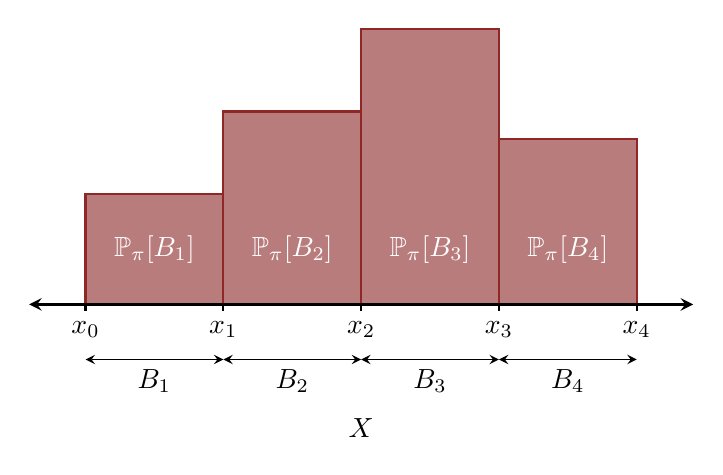
\begin{tikzpicture}[scale=0.35, thick]
  \draw [<->, >=stealth, line width=0.5] (-10, -2) -- (-5, -2)
  node[below, midway]  { $B_{1}$ }; 
  
  \filldraw [fill=mid, draw=dark] (-10, 0) rectangle (-5, 4);
  \node[text=white] at (-7.5, 2) { $\mathbb{P}_{\pi}[B_{1}]$ };
  
  \draw [<->, >=stealth, line width=0.5] (-5, -2) -- (0, -2)
  node[below, midway]  { $B_{2}$ }; 
  
  \filldraw [fill=mid, draw=dark] (-5, 0) rectangle (0, 7);
  \node[text=white] at (-2.5, 2) { $\mathbb{P}_{\pi}[B_{2}]$ };

  \draw [<->, >=stealth, line width=0.5] (0, -2) -- (5, -2)
  node[below, midway]  { $B_{3}$ };
  
  \filldraw [fill=mid, draw=dark] (0, 0) rectangle (5, 10);
  \node[text=white] at (2.5, 2) { $\mathbb{P}_{\pi}[B_{3}]$ };
  
  \draw [<->, >=stealth, line width=0.5] (5, -2) -- (10, -2)
  node[below, midway]  { $B_{4}$ };
  
  \filldraw [fill=mid, draw=dark] (5, 0) rectangle (10, 6);
  \node[text=white] at (7.5, 2) { $\mathbb{P}_{\pi}[B_{4}]$ };
  
  \draw [<->, >=stealth, line width=1] (-12.05, 0) -- +(24.1, 0);
  \node[] at (0, -4.5) { $X$ };
  
  \draw [] (-10, 0) -- +(0, -0.25)
  node [below] { $x_{0}$ };
  
  \draw [] (-5, 0) -- +(0, -0.25)
  node [below] { $x_{1}$ };
  
  \draw [] (0, 0) -- +(0, -0.25)
  node [below] { $x_{2}$ };
  
  \draw [] (5, 0) -- +(0, -0.25)
  node [below] { $x_{3}$ };
  
  \draw [] (10, 0) -- +(0, -0.25)
  node [below] { $x_{4}$ };
  
\end{tikzpicture}

\end{document}  